\documentclass[10pt]{beamer}
\usepackage[utf8]{inputenc}
\usepackage[T1]{fontenc}
\usepackage[portuguese]{babel}
\usepackage{amsmath}
\usepackage{amsfonts}
\usepackage{amssymb}
\usepackage{graphicx}
\usetheme{CambridgeUS}
\usepackage{multicol}
\usepackage{multirow}
\usepackage{array}
\usepackage{booktabs}
\usepackage{xcolor}
\usepackage{pagecolor}
\usepackage{mdframed}
\usepackage{tabularx} \newcolumntype{L}{>{\raggedright\arraybackslash}X}
	
	\newcommand{\propnumber}{} % initialize
	\newtheorem*{prop}{Proposição \propnumber}
	\newenvironment{propc}[1]
	{\renewcommand{\propnumber}{#1}%
		\begin{shaded}\begin{prop}}
			{\end{prop}\end{shaded}}
	
	
	% Definicao de novos ambientes
	\newtheorem{defn}{Defini\c c\~ao} 
	\newtheorem{teo}[theorem]{Teorema}
	\newtheorem{ex}[theorem]{Exemplos}
	\newtheorem{hint}[theorem]{Dica!}
	\newtheorem{refboi}[theorem]{Citação!}
	
	\graphicspath{{./images/}}
	
	\usebackgroundtemplate{
\includegraphics[width=\paperwidth,height=\paperheight,keepaspectratio=false, ]{BG7_dark_UFF.png}}
	
	
	
	
\begin{document}
	
\color{white}
\pagecolor{black}
	
\author{Lucas Herick P.S.}
\title{QUESTMAT:TRIVIA}
\subtitle{GAMIFICAÇÂO MB}
%\logo{}
\institute{Universidade Federal Fluminense}
\date{II ENC PIRP \ I DOC PIBID/PIRP}
%\subject{}
%\setbeamercovered{transparent}
%\setbeamertemplate{navigation symbols}{}	
	
\begin{frame}

			\begin{table}
			\begin{tabular}{ccc}
			 
			
\includegraphics[width=0.15\textwidth]{UFF_LOGO_wt.png} & 
\includegraphics[width=0.15\textwidth]{CAPES_LOGO_wt.png} &
			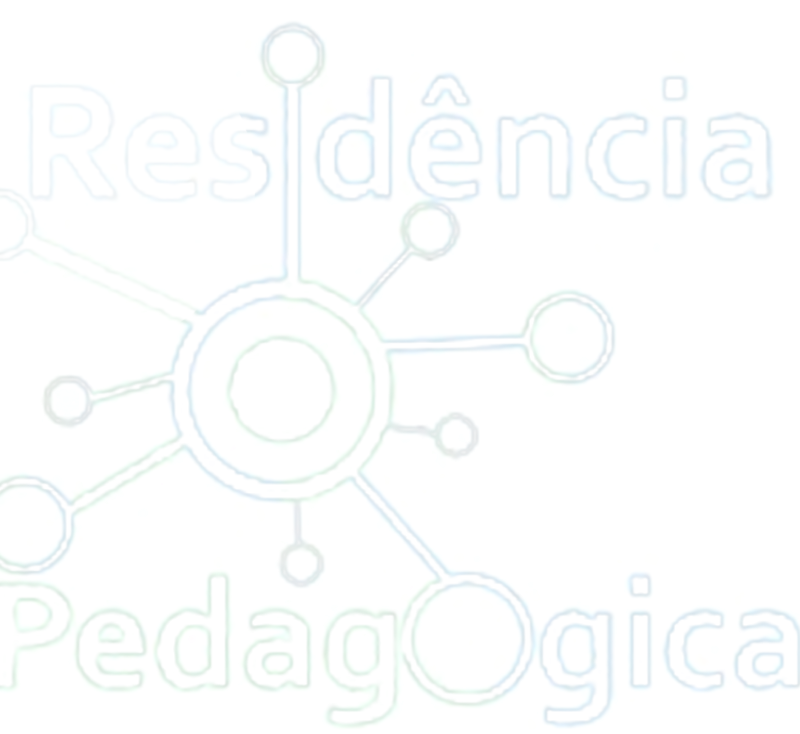
\includegraphics[width=0.15\textwidth]{PIRP_LOGO_wt.png}\\													 	     
			\end{tabular}  
   			\end{table}
 



\begin{block}{}
	
	\begin{center}
		\textbf{\large \textcolor[rgb]{1.0, 0.21, 0.37}{QUESTMAT: UMA PROPOSTA DE GAMIFICAÇÃO DA MATEMÁTICA BÁSICA}}
	\end{center}
\end{block}



\begin{center}
	LUCAS HERICK PEREIRA DA SILVA \\
	{\small FABIANO SOUZA (COORDENADOR) SANDRA WILLIAM (PRECEPTORA)\\}
	
	\vspace{5mm}
	II ENCONTRO ANUAL DO PIRP  \\ I CICLO DE FORMAÇÃO DOCENTE DO PIBID/PIRP

\end{center}

\end{frame}

%------------------------------------------------------------

\begin{frame}
\frametitle{Índice}

Esta apresentação procura introduzir a atividade QuestMat Trivia desenvolvida pelo residente Lucas Herick P.S. Aqui veremos:  \vspace{3mm} \pause

\begin{columns}

\column{0.5\linewidth}
\begin{enumerate}
	
		
		
	
	\color{white}
	
	\item Introdução
	\item Fundamentação Teórica
	\item Aspectos Técnicos
	\item Jogabilidade
	\item Roadmap
	\item Screenshots
	\item Referências Bibliográficas
\end{enumerate}

\column{0.5\linewidth}


\includegraphics[width = 0.5\linewidth]{APP_ICON_noBG.png}

\end{columns}

\end{frame}

%-------------------------------------------------------------

\begin{frame}
\frametitle{Introdução}
\begin{columns}
	\column{0.7\linewidth}

O presente instrumento - QuestMat Trivia - foi desenvolvido com o auxílio de assets em linguagem computacional C\# com o IDE Unity, que é um ambiente internaciomente conhecido como uma dos melhores softwares de desenvolvimento de jogos 2D e 3D para plataformas Windows, Linux, Android, iOS, entre outros.

	\column{0.3\linewidth}
	
	
\includegraphics[width=\linewidth]{unity.jpg}
\end{columns}

\vspace{1cm}
\begin{hint}
Nesta apresentação, você encontra todas as informações necessárias
para sua segurança e uso adequado do aplicativo em seu aparelho mobile. 
\end{hint}

\end{frame}

%--------------------------------------------------------------

\begin{frame}
\frametitle{Fundamentação Teórica}

O objetivo inicial é que alunos façam uso da aplicação para trabalho e treinamento nas categorias que sentirem maior dificuldade no meio escolar, e introduzir também um ambiente colaborativo entre docentes e discentes.
\pause 
Conforme cita (Brasil, 1998),  a gamificação de um conteúdo muito auxilia no Ensino-aprendizagem da matemática.
\pause (Grando, 2001) também cita que a gamificação também pode se tornar um eixo motivador na memorização dos conteúdos. \pause 

\begin{refboi}[(Brasil, 1998)]
	"Os jogos constituem uma forma interessante de propor problemas, pois permitem que estes sejam apresentados de modo atrativo $ (\cdots) $ possibilitam a construção de uma atitude positiva perante aos erros, uma vez que as ações sucedem-se rapidamente"
\end{refboi}

\end{frame}

%--------------------------------------------------------------

\begin{frame}
	\frametitle{Fundamentação Teórica}

De acordo com pesquisas realizadas anualmente pela StatCounter denominadas GlobalStats, os sistemas operacionais mais utilizados no mundo são o Android, sistema operacional do Google, e o Windows, sistema operacional da Microsoft. \pause


\begin{center}
	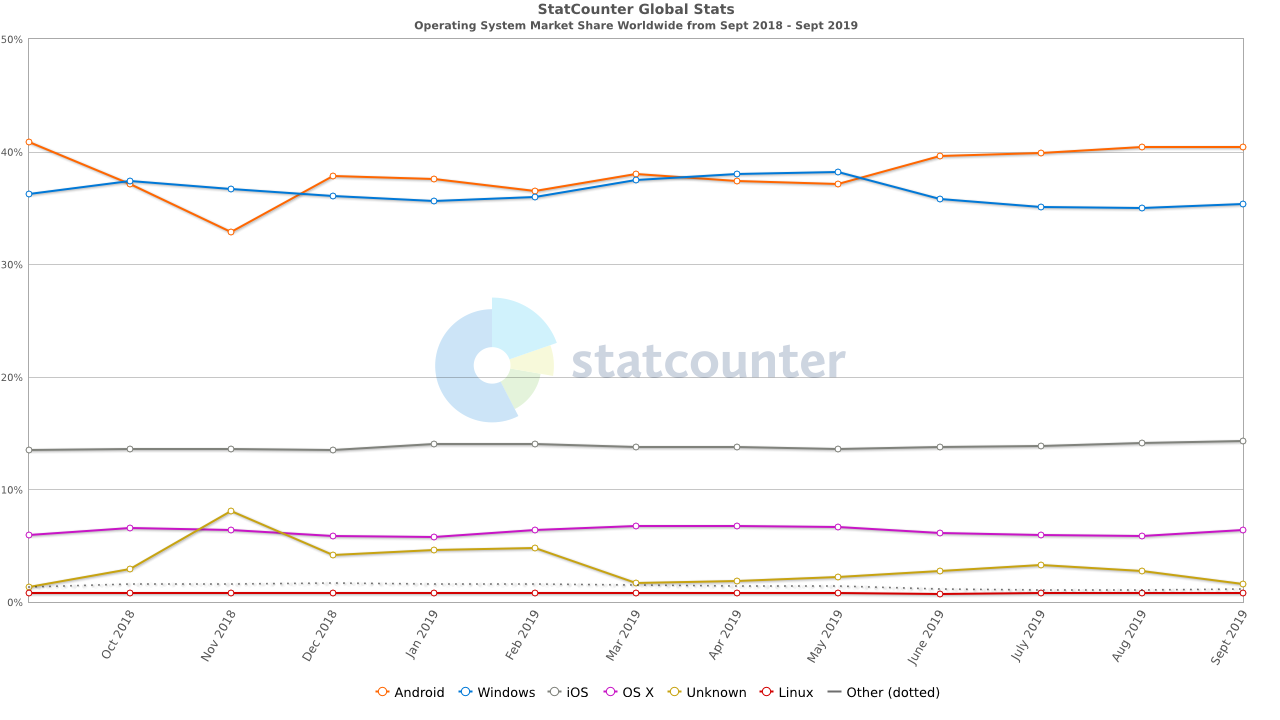
\includegraphics[width=0.8\linewidth]{StatCounter-os_research.png}
\end{center}




\end{frame}

%--------------------------------------------------------------

\begin{frame}
	\frametitle{Aspectos Técnicos}
	
	
	Com base nos dados acima, visando atingir o maior público, foram desenvolvidos versões para ambos
	os sistemas com maior público. O .apk do aplicativo funcionará em dispositivos cujo sistema operacional seja Android superior a versão 4.4 (Versão Kitkat). Já o executável (.exe) funcionará em computadores cujo sistema operacional seja Windows. \pause
	
	\begin{hint}
		Atenção! De acordo com a Sociedade Brasleira de Pediatria (SBP) e a Academia Americana de Pediatria (AAP), o tempo recomendado de observação de telas de smartphone é de até duas horas por dia. 
	\end{hint}
	
	
\end{frame}

%---------------------------------------------------------------

%--------------------------------------------------------------

\begin{frame}
	\frametitle{Roadmap}
	
  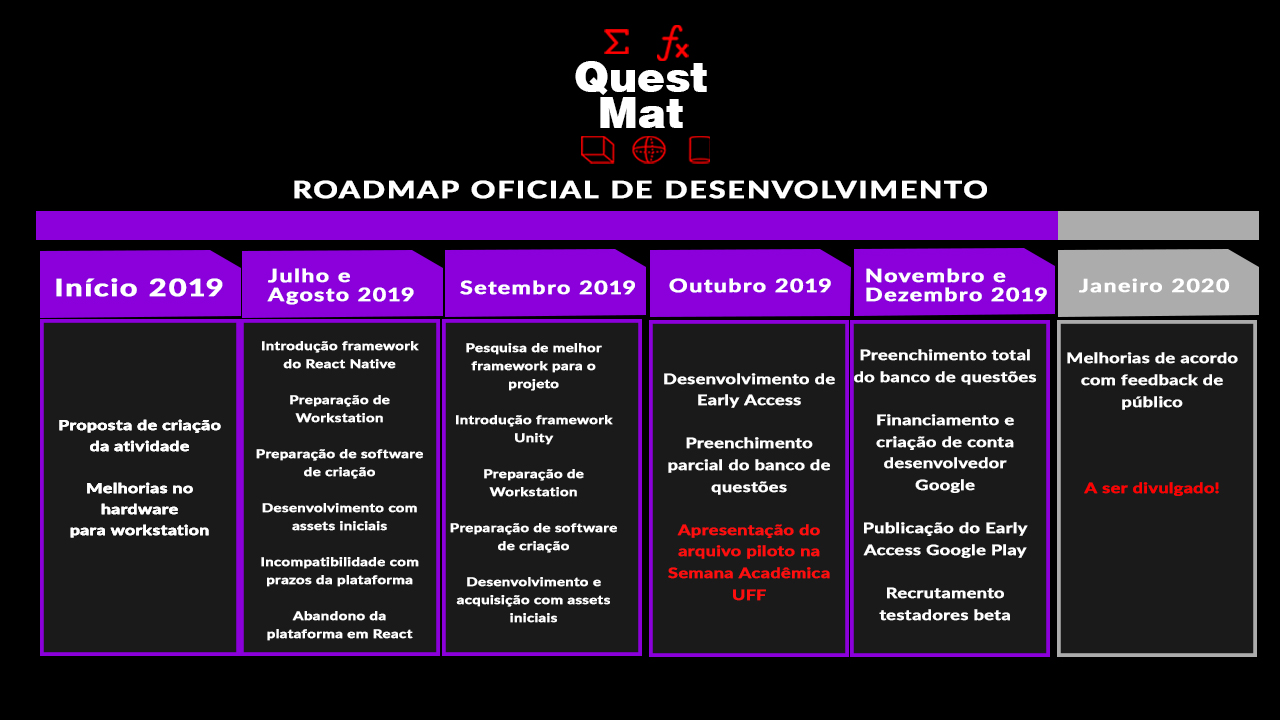
\includegraphics[width=\linewidth]{ROADMAP_QUESTMAT.jpg}
	
%%	\resizebox{\linewidth}{!}{% Resize table to fit within \linewidth horizontally
%	\begin{table}
%		\centering
%	
%	{\tiny \begin{tabularx}{\linewidth}{|L|L|L|L|L|L|L|L|}
%		\hline 
%		\multicolumn{8}{|c|}{Roadmap Oficial de desenvolvimento Questmat Trivia}\\ 
%		\hline 
%		&  &  &  &  &  &  &  \\ 
%		\hline 
%		Início 2019 & Julho / 2019 & Agosto / 2019 & Setembro / 2019 & Outubro / 2019 & Novembro / 2019 & Dezembro / 2019 & Janeiro / 2020 \\ 
%		\hline 
%		Proposta de criação da atividade & Introdução framework do React Native & Desenvolvimento com assets iniciais & Pesquisa de framework  melhor compatível com o projeto & Desenvolvimento do Early Access & Preenchimento total do banco de questões  & Recrutamento para Testadores Beta & Melhorias de acordo com feedback do público \\ 
%		\hline 
%		Melhorias no hardware para workstation & Preparação de Workstation & Incompatibilidade do prazo de entrega com plataforma & Introdução framework do Unity & Preenchimento parcial do banco de questões  & Publicação e divulgação do Early Access & Conta desenvolvedor na Google Play &  \\ 
%		\hline 
%		& Preparação de Software de criação & Abandono da criação da plataforma em React Native & Desenvolvimento / aquisição de assets necessários & Apresentação do piloto na Semana Acadêmica UFF & Recrutamento para Testadores alpha & Divulgação do app na Google Play &  \\ 
%		\hline 
%		&  &  & Mockup  &  &  &  &  \\ 
%		\hline 
%	\end{tabularx}
%	}
%\end{table}
	

	
	
\end{frame}

%---------------------------------------------------------------


\begin{frame}
\frametitle{Jogabilidade (Early Access)}

\begin{columns}
	\column{0.4\textwidth}
	
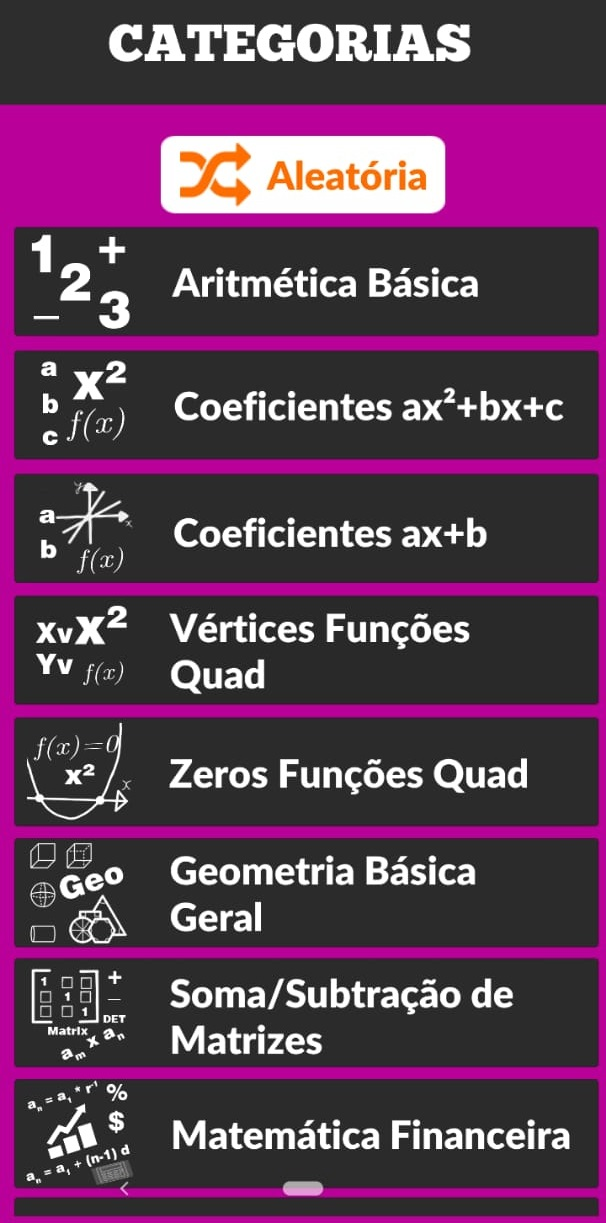
\includegraphics[width=0.9\linewidth, height=0.9\textheight,keepaspectratio=false]{quiz_selection.jpeg} \pause	
	
	
	\column{0.6\textwidth}
	

Ao iniciar o aplicativo, uma tela introdutória se abrirá. Não é necessário fazer nada ainda, apenas aguardar a tela inicial. Ao adentrar no menu inicial, estão disponíveis cinco botões de seleção sendo tres destes, métodos de jogatinas diferentes em implementação.
Em "Iniciar quiz", o usuário poderá selecionar na \colorbox{orange}{janela de seleção} um dos conteúdos previamente selecionados. 

%Conforme citado na tela de créditos 

\end{columns} 
\end{frame}

%--------------------------------------------------------------

\begin{frame}
\frametitle{Jogabilidade (Early Access)}


\begin{columns}
	\column{0.4\textwidth}
	
	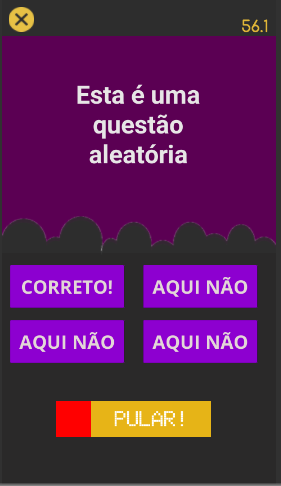
\includegraphics[width=0.9\linewidth, height=0.9\textheight,keepaspectratio=false]{questao_random.PNG} \pause	
	
	
	\column{0.6\textwidth}
	
	
Após aguardar a tela de aviso de cinco segundos, aparecerá a \colorbox{purple}{tela de questionário} no qual estará disponível uma questão para resolução aleatóriamente selecionada dentro do banco de dados do app. Dentre as quatro opções, apenas uma estará correta. (veja o exemplo ao lado). O usuário também poderá pular a questão. 
	
\end{columns}  
\end{frame}

%--------------------------------------------------------------
\begin{frame}
\frametitle{Jogabilidade (Early Access)}


\begin{columns}
	\column{0.4\textwidth}
	
	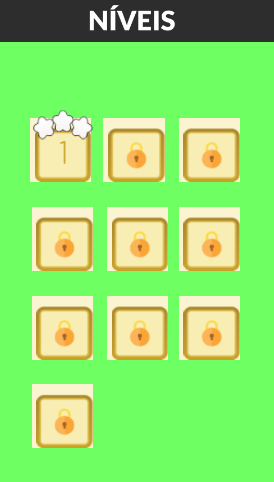
\includegraphics[width=0.9\linewidth, height=0.9\textheight,keepaspectratio=false]{challenge_levels.png} \pause	
	
	
	\column{0.6\textwidth}
	
	
	Outra seção que também se encontra em fase de implementação é a seção \colorbox{green}{DESAFIO}. O desafio é um questionário dividido em níveis que deverão ser desbloqueados, em modo carreira. O objetivo aqui é incentivar o usuário a desenvolver seu pensamento rápido pois o tempo de resolução é comparavelmente menor comparado ao quiz básico. Para prosseguir em cada nível, o usuário deve acertar 7 de 20 questões. 
	
\end{columns}


\end{frame}

%--------------------------------------------------------------

\begin{frame}
\frametitle{Screenshots}
\begin{tabular}{cccc}
	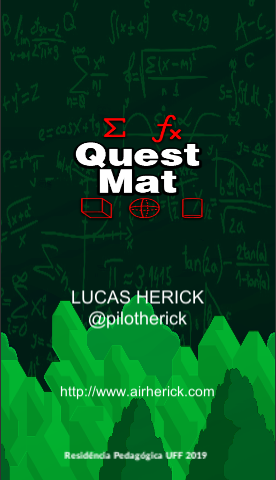
\includegraphics[width=0.22\linewidth]{QuestMat_splash.PNG} &
	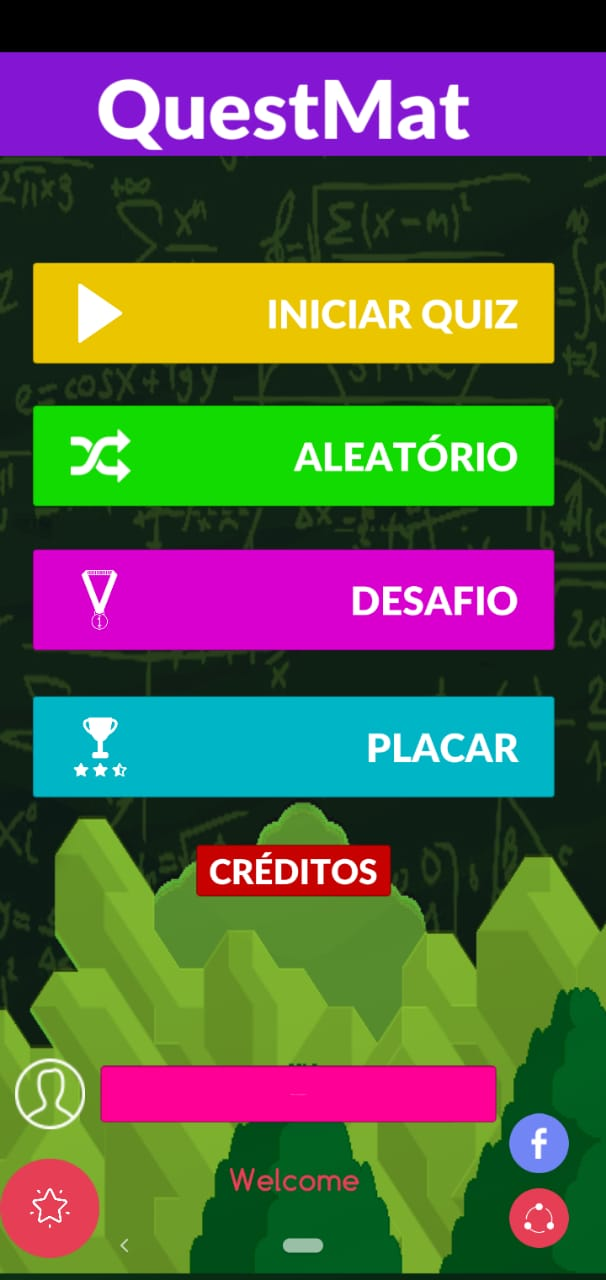
\includegraphics[width=0.22\linewidth]{menu_quest.jpeg} &
	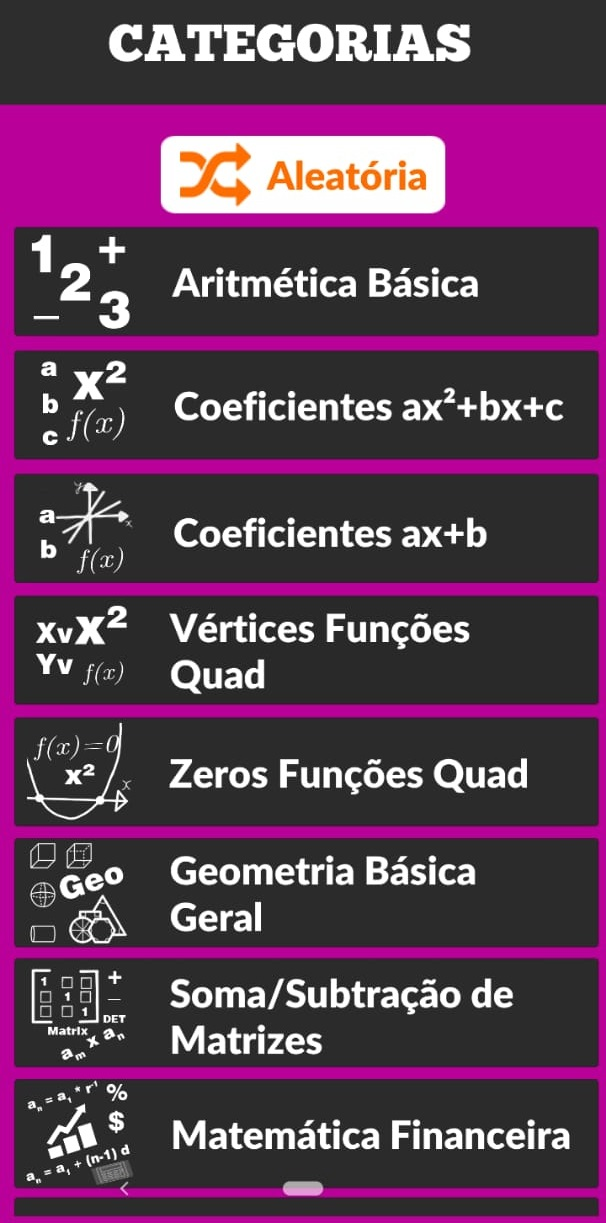
\includegraphics[width=0.22\linewidth]{quiz_selection.jpeg} &  
	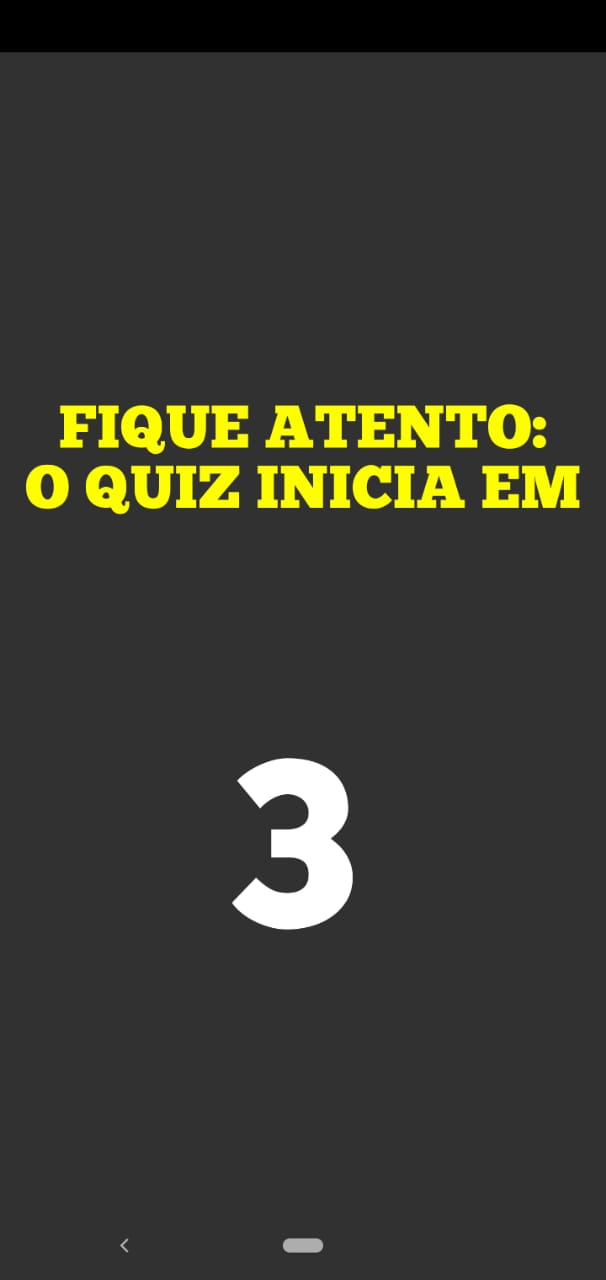
\includegraphics[width=0.22\linewidth]{timer_quest.jpeg}
%	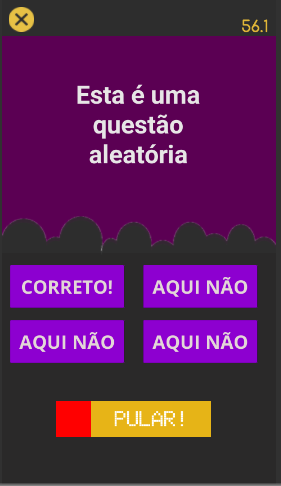
\includegraphics[width=0.15\linewidth]{questao_random.PNG}  &
%	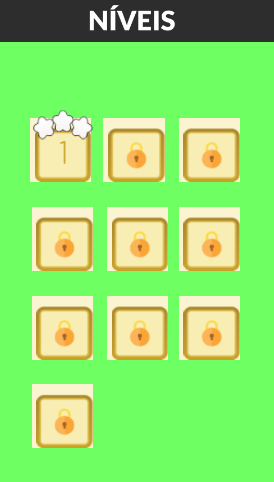
\includegraphics[width=0.15\linewidth]{challenge_levels.png}  \\  
\end{tabular} 




\end{frame}

%--------------------------------------------------------------

\begin{frame}
\frametitle{Screenshots}
\begin{tabular}{cccc}
		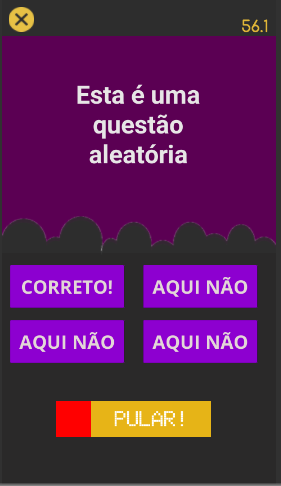
\includegraphics[width=0.22\linewidth]{questao_random.PNG}  &
		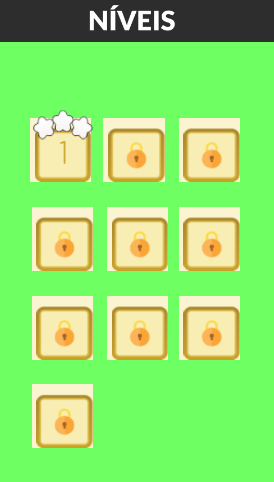
\includegraphics[width=0.22\linewidth]{challenge_levels.png}  &
		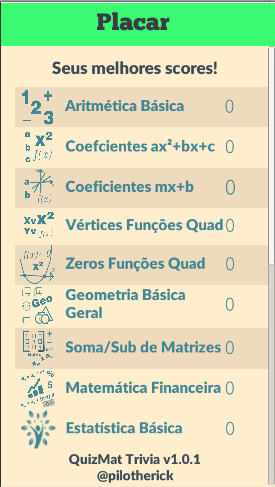
\includegraphics[width=0.22\linewidth]{scores_quest.PNG}  &
		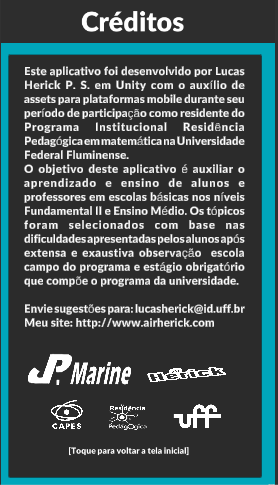
\includegraphics[width=0.22\linewidth]{credits_quest.PNG}    
\end{tabular} 




\end{frame}

%--------------------------------------------------------------

\begin{frame}
\frametitle{Time to play!}

\begin{figure}
%	\centering
	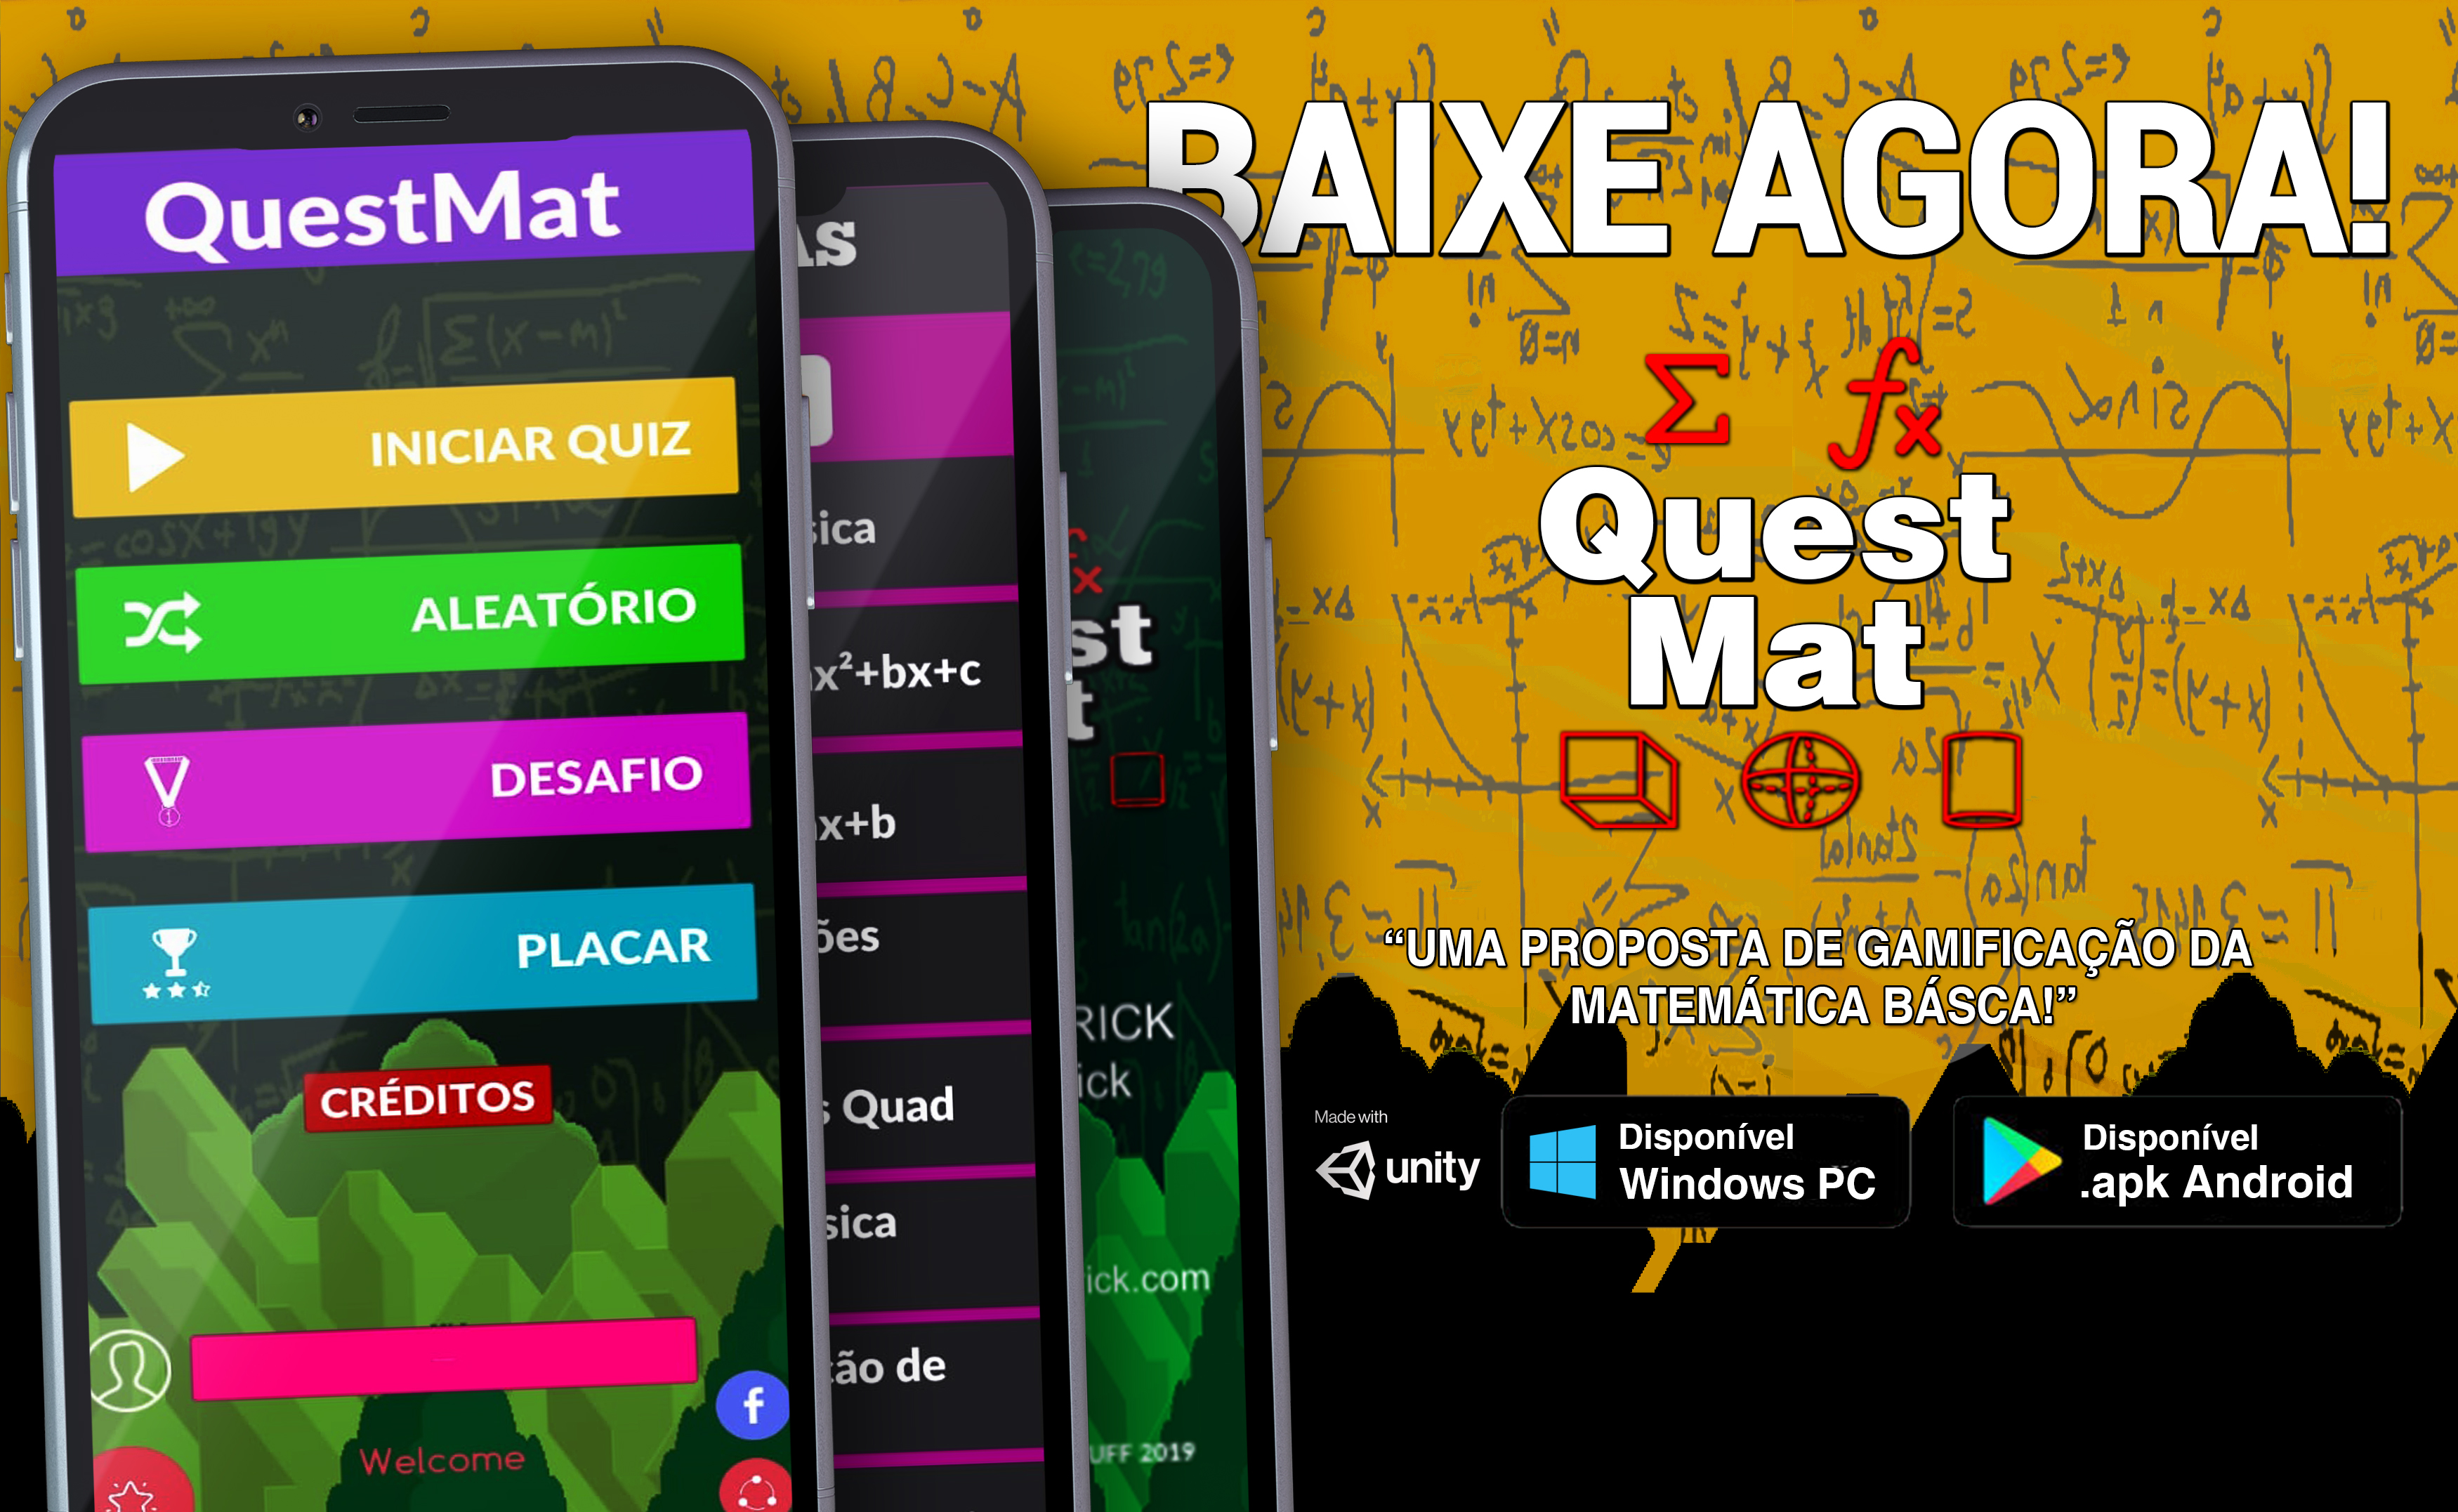
\includegraphics[width=\linewidth, height=0.70\textheight]{QUESTMAT_MOCKUP.jpg}
	\caption{\color{white}{Banner proposto para impressão: Baixe agora! (faltando QR codes )}}
%	\label{fig:questmat-appmockup}
\end{figure}

\end{frame}
%--------------------------------------------------------------


\begin{frame}
	\frametitle{Q\&A}
	
	
\begin{center}
{\Huge 	Q\&A \\
	
	\vspace{5mm}
		Perguntas e Respostas}
\end{center}
	
\end{frame}
%--------------------------------------------------------------


\begin{frame}
\frametitle{Referências Bibliográficas}

\begin{thebibliography}{llll} \color{white}{
	
	\bibitem{BRASIL} BRASIL, Ministério da Educação e da Secretaria de Educação Média e
	Tecnológica. Parâmetros Curriculares Nacionais: Matemática (PCN+). Brasília:
	MEC/SEMT, 1998. Disponível em:
	http://portal.mec.gov.br/seb/arquivos/pdf/matematica.pdf Acesso em: 02 de
	dezembro de 2018.
	
	\bibitem{GRANDO1} GRANDO, Regina Célia. O jogo e a Matemática no contexto da sala de aula.
	São Paulo: Paulus, 2004. p.115
	
	\bibitem{GRANDO2} GRANDO, Regina Célia. O conhecimento matemático e o uso de jogos na sala
	de aula. 2000. 239f. Tese de doutorado- Faculdade de Educação, Universidade
	Estadual de Campinas, Campinas, São Paulo, 2000.
	
	\bibitem{SBP}https://www.sbp.com.br/imprensa/detalhe/nid/tempo-maximo-de-uso-de-telas-para-criancas-e-adolescentes-sera-um-dos-temas-tratados-em-evento-da-sbp-a-ser-realizado-em-belo-horizonte/
	
	\bibitem{AAP}AAP, 
	https://revistacrescer.globo.com/Voce-precisa-saber/noticia/2016/10/academia-americana-de-pediatria-atualiza-recomendacao-de-tempo-de-telas-para-criancas.html
	
}

\end{thebibliography}{llll}


 




\end{frame}

%--------------------------------------------------------------
\end{document}